Automatic program synthesis has been a long term goal of the field of artificial intelligence since its inception \cite{mannaAutomaticProgramSynthesis1971}, promising to reduce the workload of software developers by automatically solving some of the tasks they face.
And since the field's inception it has been grappling with the challenging properties of the sparse optimization space \cite{alurSyntaxguidedSynthesis2013, davidProgramSynthesisChallenges2017} that is the set of all programs in a certain programming language, namely, 
\begin{enumerate}
    \item valid error-free programs constitute an exceedingly small part of the space of possible strings, so any program synthesis algorithm that incorporates random guessing (for instance, a randomly Reinforcement Learning with random initialization \cite{suttonReinforcementLearningSecond2018}) is exceedingly unlikely to guess a valid program;
    \item a small edit in a program can result in a large difference in it's behavior (and, conversely, the same algorithm can be expressed with very different programs), hence the programs we would like to find are not clustered in any compact part of the optimization space;
    \item some of the evaluation mechanisms of programs, especially in the \emph{Programmatically Interpretable Reinforcement Learning} paradigm involve stochasticity and can yield different results for the same program.
\end{enumerate}

In other words, the search space in program synthesis is \emph{sparse}, \emph{brittle} and sometimes \emph{noisy} \cite{arnoldNoisyOptimizationEvolution2002} - all known challenges in Optimization Theory.

\newpage
\section{Genetic programming}

\begin{figure}[H]
    \centering
    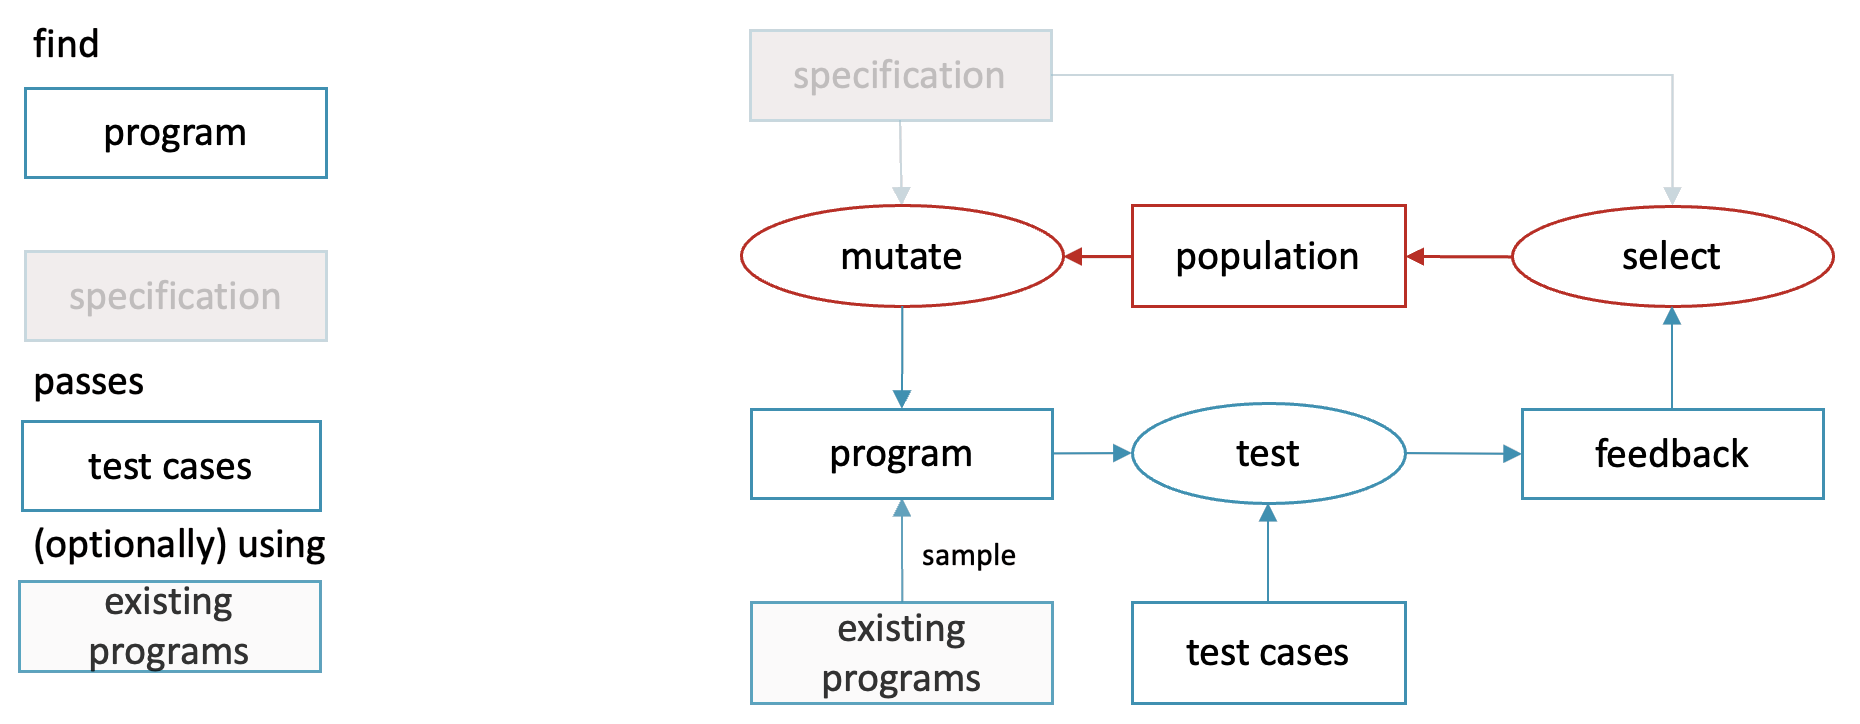
\includegraphics[width=\linewidth]{gp.png}
    \caption{Genetic Programming, schematic definition}
    \label{fig:gp}
\end{figure}

The family of optimization methods best applicable to this type of complex non-differentiable search space is \emph{genetic and evolutionary methods} - biologically inspired methods that operate on a population of candidate solutions (programs), randomly edit (\emph{mutation}) and combine (\emph{recombination}) to expand the population and the prune the population by \emph{natural selection}: removing the candidates that adhere to the specification the least.
In an evolutionary setting, if at least one (preferably several) valid program is known, initializing the population to include them drastically speeds up the search process, thus addressing the sparsity issue.

\newpage
\section{Constrained programming languages}

\paragraph{Logic programming}

Instead of (or in addition to) generating a program first and testing whether it adheres to specification, \emph{deductive} methods apply equivalence rules to translate the specification into an executable.
This is hard to apply in \emph{programmatically interpretable reinforcement learning} where the specification is a black box, but can be a powerful approach in \emph{code translation} and \emph{programming by example} paradigms.

\paragraph{Domain specific languages}

\newpage
\section{Pre-training methods}

\emph{Inductive synthesis}

\emph{concept space}

The paradigm of foundation models \cite{foundation-models} has recently been very prominent in machine learning and machine learning on source code is no exception.
In this paradigm, a model is first trained on a large dataset to solve a generic task such as next-token prediction and then used as a central component in solutions of various specific tasks.
The foundation models for source code, based on architectures such as GPT Codex \cite{radfordImprovingLanguageUnderstanding,chenEvaluatingLargeLanguage2021,codegen,gpt-neo} and BERT \cite{devlinBERTPretrainingDeep2019,codebert} have enabled significant process in tasks like programming by example \cite{halbertProgrammingExample1984} and even human-comparable performance in coding competitions \cite{liCompetitionLevelCodeGeneration2022}.

\paragraph{Autoregressive models}


\paragraph{Autoencoder models}

While undoubtedly useful in many program synthesis tasks, popular foundation models may fall short in the areas of genetic programming \cite{genprogast} and genetic improvement of software \cite{petke2018:genetic}.
In this settings, new programs are found by exploring the space of programs similar to one or several reference programs.
The task of applying these perturbations to programs could benefit from a foundational model, however, it's unclear how to achieve this with the current autoregressive models.
Autoencoder Genetic Programming \cite{autoenc-gp,denoising-autoenc-gp,latentspaceopt} argues for using autoencoder \cite{autoencoders} models instead.
These models embed programs into a high-dimensional vector space, making it easy to mutate a program by add random noise to the embedding vector or combine several programs by averaging their embedding vectors.

\newpage
\section{Grammar guided synthesis}

Another way to constrain the hypothesis space is to use the grammar of the programming language in question directly in the program generation process.

Unlike natural languages, programming languages are easier to represent structurally due to the nature of their syntax which improves machine learning performance.

\section{Human in the loop}

\paragraph{Completion}

\paragraph{Sketching}

\section{Open problems}

Most open problems lie in the domain of \emph{Programmatically Interpretable Reinforcement Learning}

However, a fully autonomous system for Programmatically Interpretable Reinforcement Learning is yet to be devised. In chapter \ref{ch:bfpp}